Dans le premier et le deuxième rapports, nous avions présenté notre solution IoT orientée Smart Health, afin de résoudre le problème de congestion des hôpitaux dans les services de soins intensifs. Plus précisément, nous avions proposé les dispositifs et les protocoles de communication et de réseau (rapport 1) ainsi que le middleware (rapport 2) de notre solution. Enfin, nous avions abordé les enjeux liès à la QoS, et à la sécurité et la privacité de notre solution.
\\

Le présent rapport a permis quant à lui de présenter les différents services de la couche applicative de notre solution, à travers différents points de vue, comme ceux du personnel médical, du personnel de maintenance, des proches du patient, de l'hôpital, et de l'architecture. Le but étant également de faire en sorte que ces services respectent certains requis en vue de répondre correctement à la problématique de congestion de l'hôpital dans le secteur des soins intensifs. 

Aussi, dans ce rapport, nous avons abordé les problèmes liés à la Qalité de Service (QoS), et à la sécurité et privacité de notre solution, et ce à travers les différentes couches de notre système (dispositifs et protocoles de communication, middleware, et services). La figure \ref{final} permet d'avoir une vue d'ensemble de ce qui a été abordé, analysé, et conceptualisé dans ce rapport.
\\
\begin{figure}[h!]
	\hspace*{-4.2cm}
	\centering
	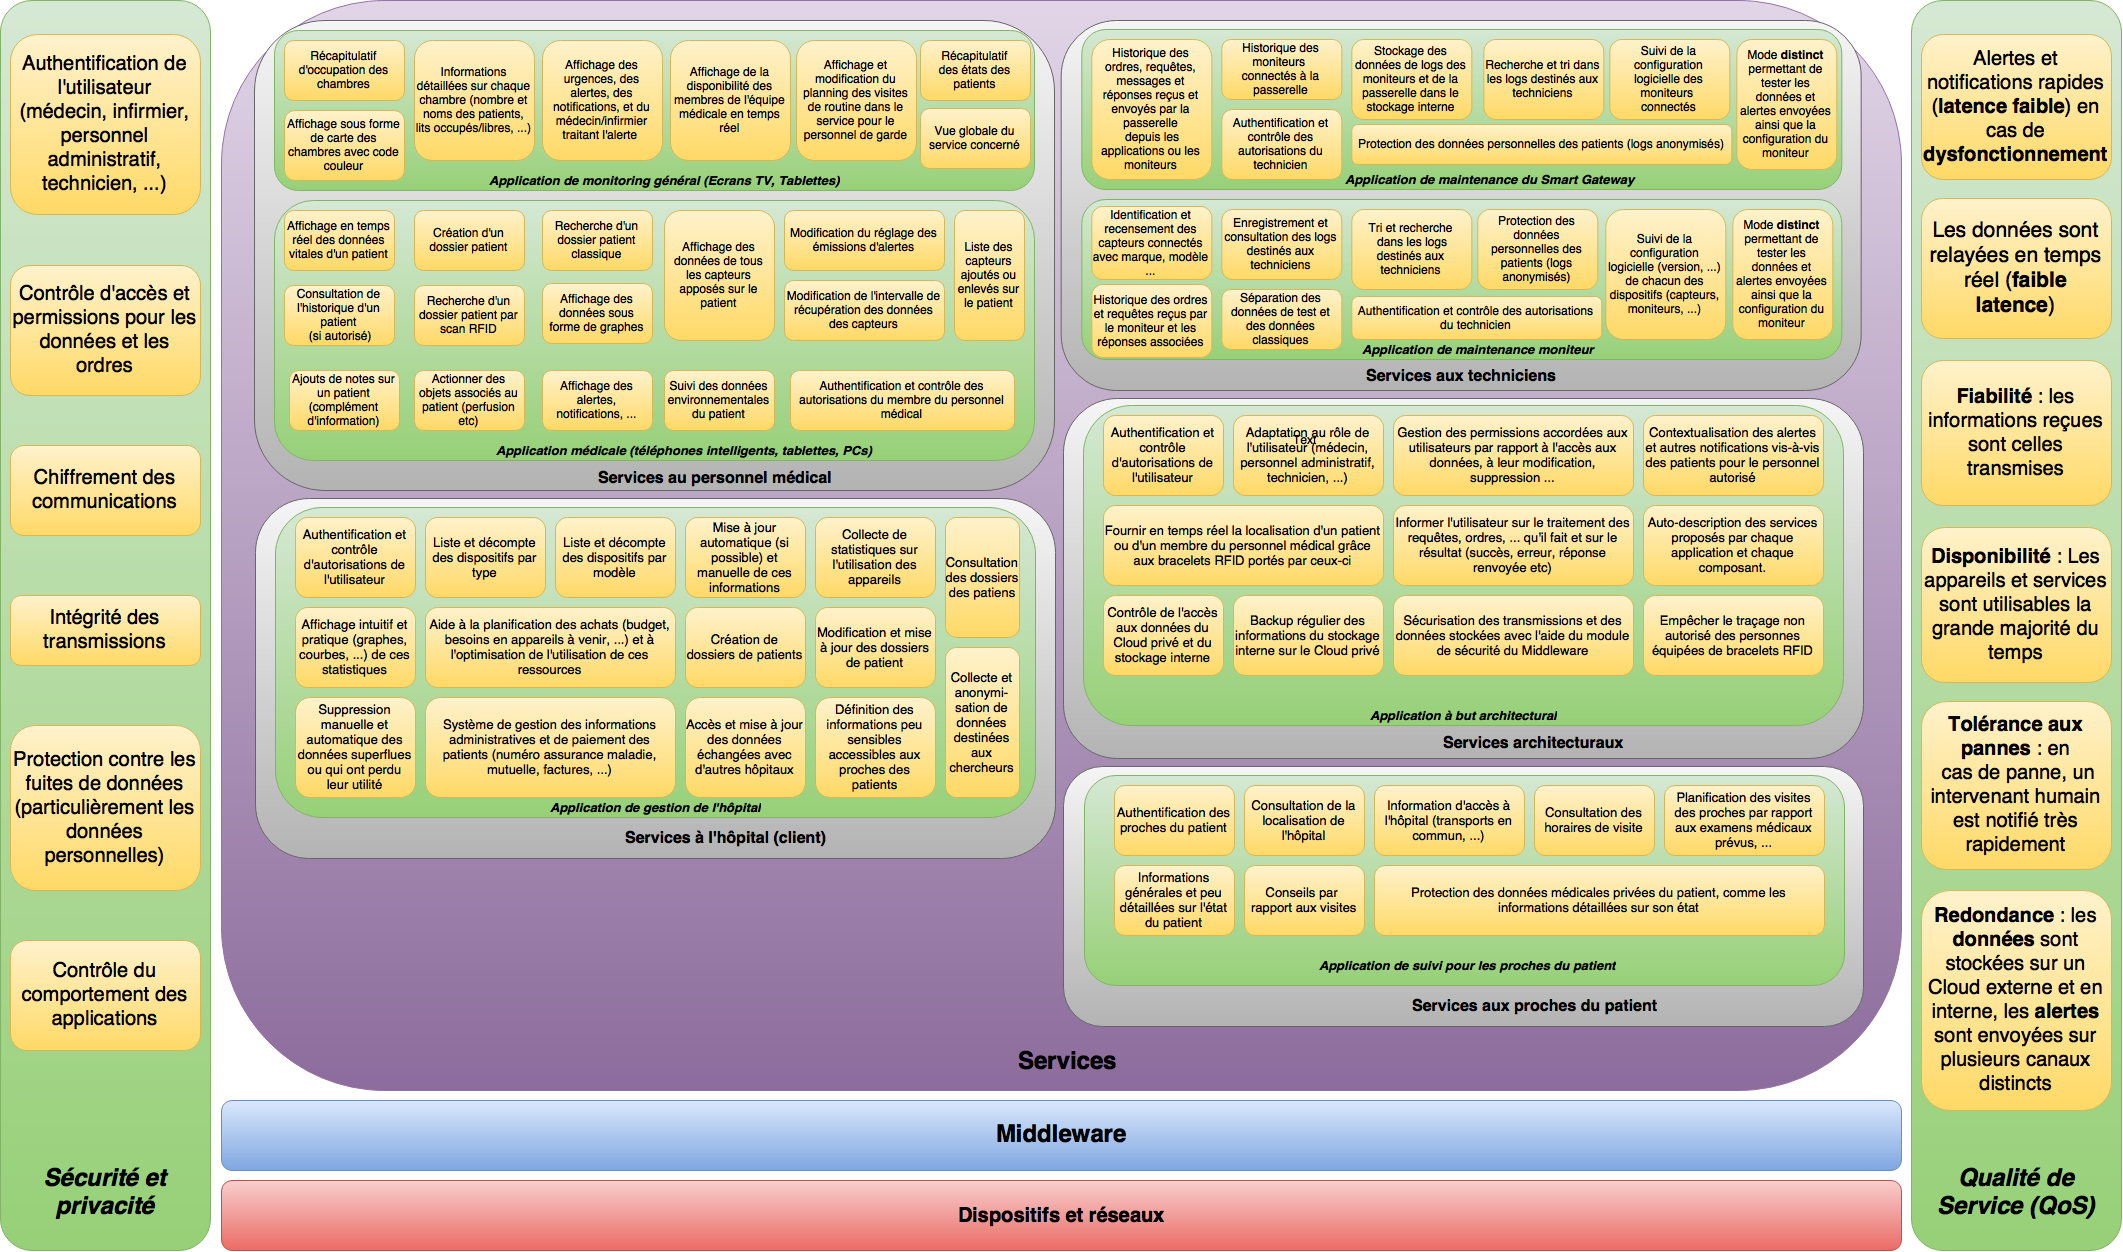
\includegraphics[width=1.7\textwidth]{final.png}
	\caption{Services proposés par notre Solution (Couche Applicative), QoS, Sécurité et Privacité}
	\label{final}
\end{figure}

Par la suite, l'objectif sera de présenter en classe notre solution, notamment au niveau de son architecture, et de mettre en contexte les problématiques de QoS, et de confidentialité et de sécurité.